\chapter{Introduction}\label{chap:intro}
The existence of planets orbiting other stars different from our Sun, lived in the human imagination for centuries. During the sixteenth century, the Italian philosopher Giordano Bruno suggested, for the first time in history, that more planet could be outside the Solar System. Even though the first claims of exoplanet detection began at the end of the nineteenth century, it was not until more than four hundred years after the statement of Giordano Bruno, that the first exoplanet was confirmed in 1992. Surprisingly, it was not just one exoplanet but three, orbiting the pulsar PSR B1257+12 more than 1000 light-years away from us. Today, more than 4,000 exoplanet are confirmed, and thousands more are waiting for their confirmation.

The increasing number of discovered exoplanets have been reached thank to two techniques: Radial Velocity and Transits. Each one of these techniques had their own advantages depending on the physical properties of the planetary system. When the orbit of the exoplanet is aligned with the line of sight from Earth, the pass of the planet in front of its host star causes that the star's flux decreases proportionally to the size of the planet. Thus, its radius, in comparison with the radius of the star, can be determined directly using the Transit method. In the other hand, the gravity due to the presence of a planet will set the center of mass of the system, in a place different from the star's center. Therefore, the star will move in its own small orbit with a size proportional to the mass of the planet. In this case, the Radial Velocity method unveils the planet's minimum mass ($M_{p}\sin i$). The perfect scenario comes when both methods can be used in the same planetary system, allowing to derive essential properties such as the real mass and the mean density of the planet.


\section{Transiting Exoplanets}
The Transit method is today the most successful technique to discover extrasolar planets (see Fig.~\ref{amount_exoplanet}). The Kepler mission was launched in 2009 and during its almost nine years of provided thousands of discoveries due to this method.

\begin{figure}[H]
\centering
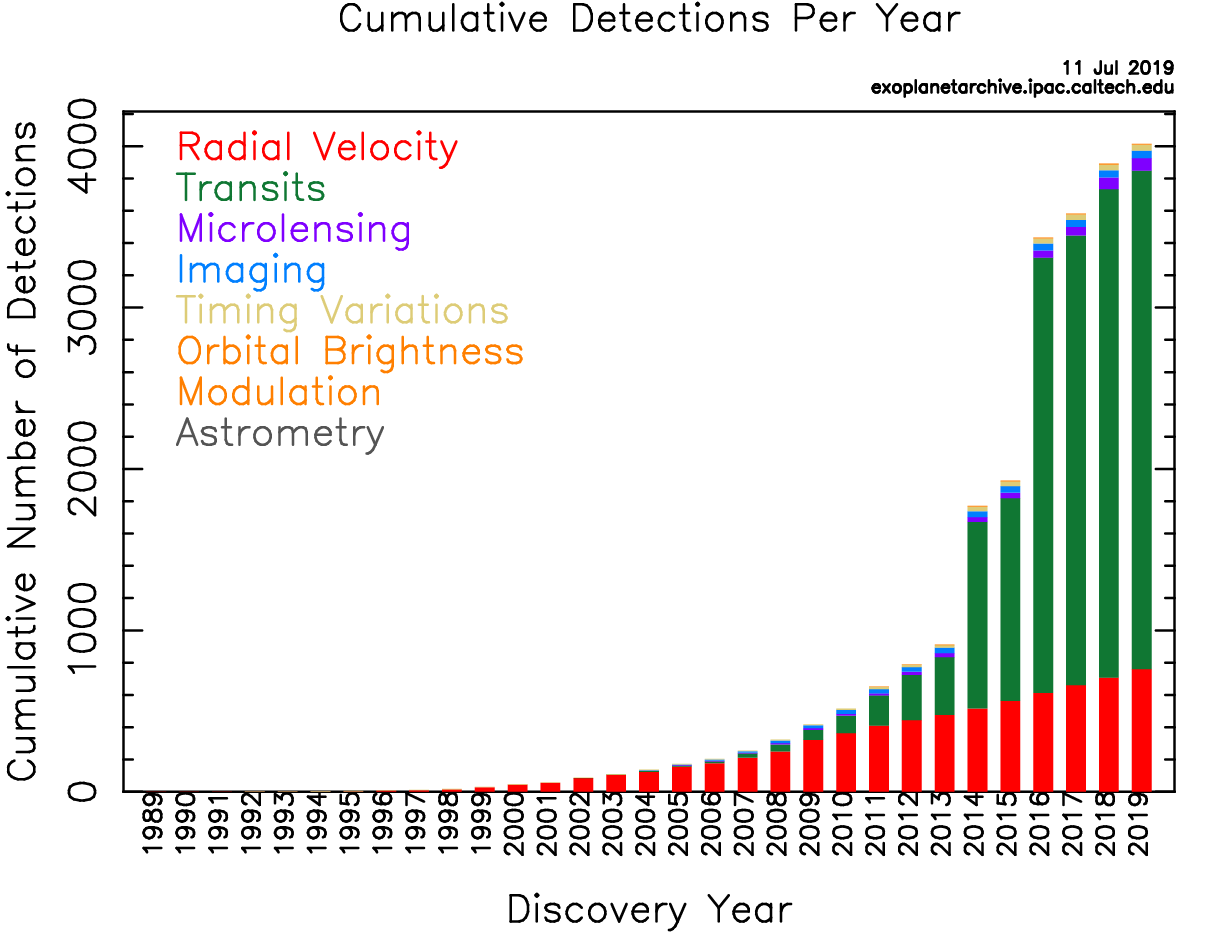
\includegraphics[width=0.7\columnwidth]{imagenes/exo_dischist_cumulative.png}
\caption{Accumulative number of discovered exoplanets by year.}
\label{amount_exoplanet}
\end{figure}

The light curve produced by a transit event provides important information of the planetary system. For example, it is the only way on which we can derived directly the proportion between the exoplanet and star radius. It can also give information about the impact parameter, and therefore, the inclination of the orbit. 

In Figure~\ref{transit} is described the architecture of a transiting exoplanet. Thanks to its geometry, the transit event as well as some parameters of the planetary system can be described with a few simple relations (cite Seager and Mallean y Winn).  When the planet passes in front of its star produced a dimming in its flux called primary transit. The maximum drop during the transit event defines the transit depth $\Delta{F}$:

\begin{equation}
    \Delta{F} = \left(\frac{R_{p}}{R_{*}}\right)^2 
\end{equation}

Where $R_{p}$ and $R_{*}$ are the planet and star radius, respectively. The numbers 1, 2, 3 and 4 correspond to the contact times: $t_{1}$, $t_{2}$, $t_{3}$ and $t_{4}$. The total duration of the transit is $t_{T} = t_{4}-t_{1}$ and the full duration is $t_{F}=t_{3}-t_{2}$. The total duration of the transit can be also described considering planetary parameters such as the period $P$, semi-major axis $a$ and orbital inclination $i$:

\begin{equation}
    t_{T} = \frac{PR_{star}}{\pi a} \sqrt{\left(1+\frac{R_{p}}{R_{*}}\right)^2-\left(\frac{a\cos i}{R_{*}}\right)}
\end{equation}

The impact parameter $b$, is the sky-projected distance between the center of the star and the planet at conjunction:

\begin{equation}
    b = \frac{a\cos{i}}{R_{*}}\left(\frac{1-e^2}{1+e\sin{\omega}}\right)
\label{impact_param}
\end{equation}

Where $\omega$ is the periastron longitude. In the case of circular orbits, the eccentricity is zero, thus Eq.~\ref{impact_param} is simplified to:

\begin{equation}
    b = \frac{a\cos{i}}{R_{*}}
\label{impact_param_simple}
\end{equation}

\begin{figure}[H]
\centering
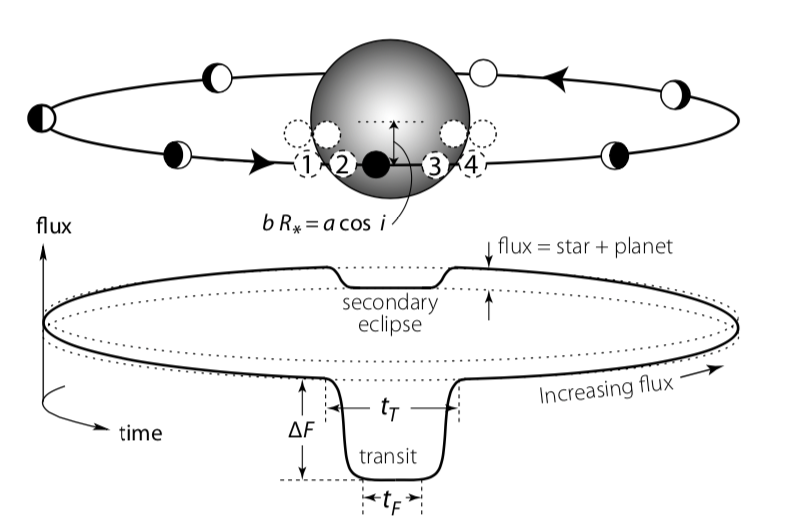
\includegraphics[width=0.8\columnwidth]{imagenes/transit.png}
\caption{Architecture of a transiting exoplanet and the observed light curve. Based on the light curve itself it is possible to measure the transit depth $\Delta F$, the impact parameter $b$. From them, the planet-to-star radius ratio $R_{p}/R_{*}$ and the orbital inclination $i$ can be derived. Figure from The Handbook of Exoplanets by M. Perryman.}
\label{transit}
\end{figure}

Depending on the orbital and physical parameters of the exoplanet, the shape of the observed light curve will vary. For example, Figure \ref{transit_examples} shows how the light curve reflects the configuration of the system. Hot Jupiters are the kind of planet easier to detect, since their planet-to-star radius ratio is larger. But an smaller planet orbiting a dwarf star could produce a similar ratio of the radius. In the other hand, exoplanets with larger orbital inclinations will produce shorter drops in the flux, in comparison with planets in the same orbital-plane with the host star.

TO DO: Add studies about transmission spectroscopy.            

\begin{figure}[H]
\centering
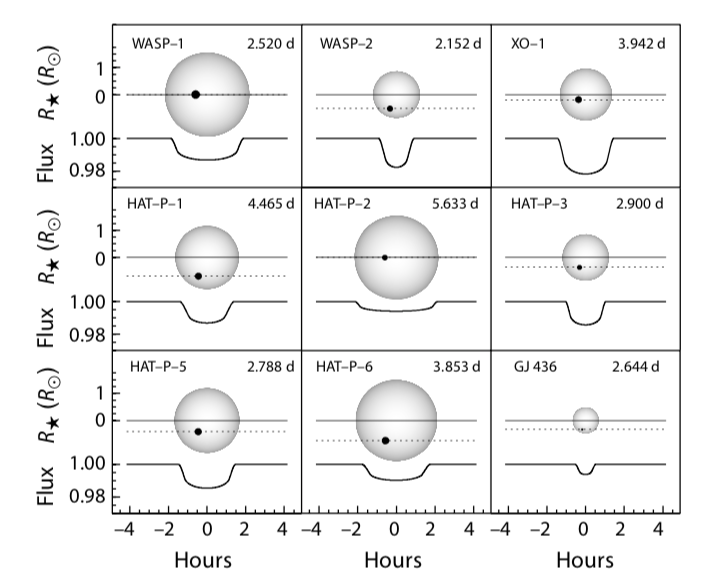
\includegraphics[width=0.8\columnwidth]{imagenes/transit_examples.png}
\caption{Examples of transiting exoplanets and how their light curves differ between them thanks to the physical properties of the exoplanet.}
\label{transit_examples}
\end{figure}


\section{Transit Timing Variations}

Since the discovery of the first exoplanet, one of the principal questions that arose was: are they alone in their systems? The idea of multiplanetary system is a consequence of our knowledge about the planetary system where we live in, and until today the Solar System has the larger number of orbiting planets. Besides the Solar System, Kepler-90 has the same number of confirmed exoplanets: eight. Statistically, around a 20\% of the confirmed exoplanets live in a multiplanetary system, but this number is theoretically larger (cite). 

The Transit Timing Variations (TTV) technique was first proposed as a way to detect Earth-mass planets in multiplanetary systems due to gravitational interactions with a transiting exoplanet \citep{Holman2005,Agol2005}. However, TTVs can be also use to measure tidal interactions between the planet and the star or to detect exomoons \citep{Kipping2009a,Kipping2009b}, among others. 

For a given light curve of a transiting exoplanet (see Fig. \ref{transit}), the transit time $T_{c}$ (or central time of the transit) is computed as:

\begin{equation}
T_{c} = \frac{t_T}{2}
\end{equation}

A single transiting planet will stay in a Keplerian orbit around its host star, producing a transit time strictly periodic. Thus, the transit time $T_c$ follows a linear function of the orbital period $P$: 

\begin{equation}
T_{c}(E) = T_{0} + E \cdot P
\label{linear_ephemeris} 
\end{equation}

Where $T_0$ is a reference transit time and $E$ is the number of epochs since $T_0$.  The presence of a second planet produces transits no exactly periodic, hence Eq.~\ref{linear_ephemeris} will not be valid. As the transit times will be no longer a linear function,  the time between  transits varies.  The variation in time produced by the perturbing body depends on the mass and geometry of their orbits. The magnitude of this variation between successive transits of the transiting planet is:

\begin{equation}
\Delta t = \frac{45\pi}{16} \frac{M_2}{M_*} P_{1} \alpha^3_{e} (1-	\sqrt{2}\alpha^{3/2})^{-2}
\label{delta_t}
\end{equation}

Where $\alpha_e = a_1/(a_2(1-e_2))$ is the ratio of the semi-major axis of the planets, considering a nonzero eccentricity for the perturbing planet ($e_2 \neq 0$) and $a_1 < a_2$. The semi-major axis of the transiting exoplanet is $a_1$ and its orbital period $P_1$, while the perturbing planet has a mass $M_2$, semi-major axis $a_2$, orbital period $P_2$ and eccentricity $e_2$. Assuming that the orbital parameters of the known transiting exoplanet are already derived from its light curve, the orbital parameters and mass of the hypothetical pertuber can be estimate numerically \citep{Nesvorny2008,Nesvorny2009}, even if the second planet does not transit the star. 

The TTV method is a efficient tool to search for additional unseen companions, since in order to employ this technique only photometry of the transiting exoplanet during a transit events is required. Moreover, this technique enhances its sensitivity when the two bodies in the system are close to Mean Motion Resonances (MMR) \citep{Agol2005,Steffen2005,Agol2007} (see Figure~\ref{rms_ttv_amplitude}) . 

\begin{figure}
\centering
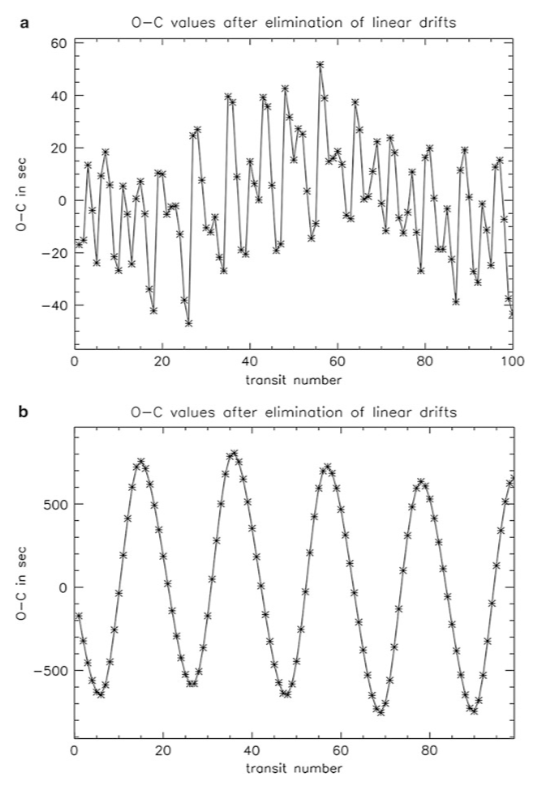
\includegraphics[width=0.6\columnwidth]{imagenes/rms_ttv_amplitude}
\caption{Example of a system with a transiting exoplanet of $1~M_{J}$ in a 10-day orbit, around a star with $0.367~M_{\odot}$. The perturber is a Earth-mass planet. Panel \textbf{a} is an O-C diagram showing the measured TTV when the pertuber has a period of 16.11 days, not in Mean Motion Resonance with the transiting planet. Panel \textbf{b} shows the TTV when the transiting planet and the perturbing planet are near an interior 2:1 resonance. The amplification of the TTV signal is by an order of magnitude. (Figure from \cite{Haghighipour2011})}
\label{rms_ttv_amplitude}
\end{figure}

\cite{Holman2010} presented the first multiplanetary system confirmed using the TTV method: Kepler-9b and Kepler-9c. 

The no detection of TTV is also important: architecture of the system.








\section{This work}

This thesis is an extension of the Transit Monitoring in the South project (TraMoS, see Chapter\ref{chap:tramos}) started in 2008 by Sergio Hoyer and Patricio Rojo. I selected a new sample of transiting exoplanets, all of them hot Jupiters without any companions detected to date.  